\documentclass[11pt]{jsarticle}

\usepackage{SPR}

\headerSPR
\begin{document}
	\titleSPR{\number\year}{\number\month}{\number\day}{D2}{吉田 皓太郎}
%%%%%%%%%%%%%%%%%%%%%%%%%%%%%%%%%%%%%%
	\articleSPRabst
		\begin{itemize}
			\item 機械学習を用いたカップ形状の設計支援
			\item 着後形状予測のためのカップの変形解析
		\end{itemize}
		
		
	\articleSPRobj
		\begin{enumerate}
			\item 定性的な機能要求を満たせるようなカップ形状を設計できる
			\item 布の物性とカップのパターンがどのような結びつきを持っているかを調べることができる.
		\end{enumerate}
%%%%%%%%%%%%%%%%%%%%%%%%%%%%%%%%%%%%%%
% 1.前回からのノルマ
	\articleSPRitemsone
		%\begin{enumerate}
		%	\item A
		%\end{enumerate}
		
		\tableofcontents
		
		
%%%%%%%%%%%%%%%%%%%%%%%%%%%%%%%%%%%%%%
%\begin{itemize}
%	\item 新規手法について
%	\item ISFAアウトライン
%\end{itemize}
%%%%%%%%%%%%%%%%%%%%%%%%%%%%%%%%%%%%%%
% 2.具体的な成果
	\articleSPRitemstwo
	\renewcommand{\labelitemi}{$\blacktriangledown$}
%%%%%%%%%%%%%%%%%%%%%%%%%%%%%%%%%%%%%
	\section{研究進捗について}
		先週の研究成果等について報告いたします.
		\begin{itemize}
			\item 機械学習を用いたシステムの概要についての試行錯誤まとめ
			\item 可展面研究調査
			\item これからのTodo
		\end{itemize}
	\section{機械学習を用いたシステムの概要についての試行錯誤まとめ}
		\subsection{進捗}
			データを作るプログラムにいくつかのバグを見つけ,それを修正しつつ,以下のような制約を$S_{const,i}  $,$ V_{const,i} $を変化させながら訓練データを作成しました.
			\begin{equation}\label{eq:size_ineq}
				S_{cup} < S_{const,i}
			\end{equation}
			\begin{equation}\label{eq:volume_ineq}
				V_{cup} < V_{const,i}
			\end{equation}
			また,手法において,$ s=0,length_L $では母線が定義できないことから,このデータを学習データから取り除くことで,精度向上を図った.
		\subsection{結果}
			入力におけるガウス過程のカーネル関数には,以下のようなRBFカーネルを用いて,得られるハイパーパラメータ$ \theta_1,\theta_2,\sigma^2 $をパラメータとして用いた.
			\begin{equation}\label{eq:RBF_Kernel}
				k(x,y) = \theta_1 \exp\left( -\frac{(x-y)^2}{\theta_2} \right)
			\end{equation}
			また,入出力に対応するガウス過程におけるカーネル関数を,次式のようなRBFカーネルと線形カーネルを,組み合わせた形で設定しました.
			\begin{equation}\label{eq:KernelForExperiment}
				k(\bd{x},\bd{y}) =  \sum_{p=1}^{N} \sigma^2 \exp\left(-\frac{(x_i-y_i)^2}{\theta_{p,r}^2}\right) + \sum_{p=1}^{N} \theta_{p,l} x_p y_p
			\end{equation}
			
			
			学習データは1800個程度あり,これを
			\begin{itemize}
				\item 学習用データ 1300個
				\item 検証用データ 500個
			\end{itemize}
			に分けて,検証を行いました.
			\bfig[H]
				\centering
				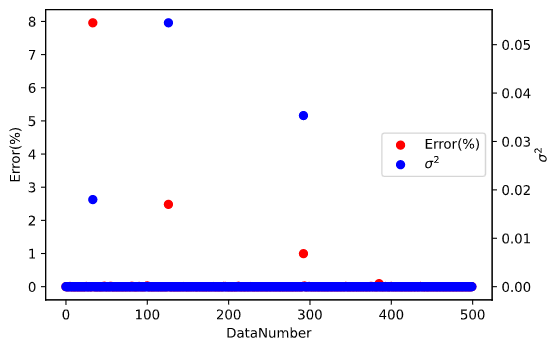
\includegraphics[scale=0.4]{./figure/ErrorVerificationDataAndVarinace.png}
				\caption{Error of Output Data and Its Variance}
			\efig
			
			ただし,誤差の単位は($ \% $)です.このモデルにおける決定変数はほぼ1であり,二乗平均平方根誤差(RMSE)は0.006であり,最大誤差はおよそ8$ \% $でありました.ガウス過程を用いるメリットとして,出力解の予測精度を大まかに表してくれるというメリットがあります.この図の通り,実際に事後分散が大きいところと,誤差の大きいところの傾向が似ていることが見て取れるかと思います.
			
			学習データの総数が増えたこともありますが,プログラムのバグ等があってうまく行えていなかった部分を修正したのが一番大きいと思われます.
			
			上記のことを通して,本研究の妥当性が確認できたのではと考えられます.
	\section{可展面研究調査}
		適用されている範囲
			\begin{itemize}
				\item 建築
				\item 航空関係(宇宙関係?)
				\item 船舶
				\item 医療機器(たぶん円錐形状とか?)
				\item 車体
				\item レーザー成形?
			\end{itemize}
		などが挙げられるようです.		
		
	\section{これからのTodo}
			\begin{itemize}
				\item データを作り直し,二枚接ぎカップ全体で学習用データを作りたい.
				\item 機能の値にしたがって解が出てくるような手法,深層学習の適用
			\end{itemize}
			
	\newpage
\vspace{10cm}
%%%%%%%%%%%%%%%%%%%%%%%%%%%%%%%%%%%%%%
% 3.達成できなかったこととその問題点
	%\articleSPRthree
	
%%%%%%%%%%%%%%%%%%%%%%%%%%%%%%%%%%%%%%

\vspace{14cm}
%%%%%%%%%%%%%%%%%%%%%%%%%%%%%%%%%%%%%%
	\articleSPRfour
	\articleSPRfive
\end{document}
